\documentclass{article}

\usepackage[a4paper,left=18mm,right=18mm,top=20mm,bottom=18mm]{geometry}
\usepackage[italian]{babel}

\usepackage{titling}
\usepackage{graphicx}
\usepackage{subcaption}
\usepackage{float}
\usepackage{hyperref}

\title{Requirements for Software engineering project}
\author{Nicolas Anselmi, David Guzman Piedrahita and Marco Vinciguerra}

\begin{document}
\maketitle
\section{Introduzione}
Per quanto riguarda la product conformance si fa riferimento al seguente link: \url{https://www.geeksforgeeks.org/iso-iec-9126-in-software-engineering/}
\\Esso si basa sui 4 seguenti principi:
\begin{itemize}
    \item \textbf{Part 1: "Quality model"} 
    \item \textbf{Part 2: "External metrics"} 
    \item \textbf{Part 3: "Internal metrics"} 
    \item \textbf{Part 4: "Quality in use metrics"} 
\end{itemize}
Per chiarire meglio il concetto si fa riferimento al seguente grafico:
\\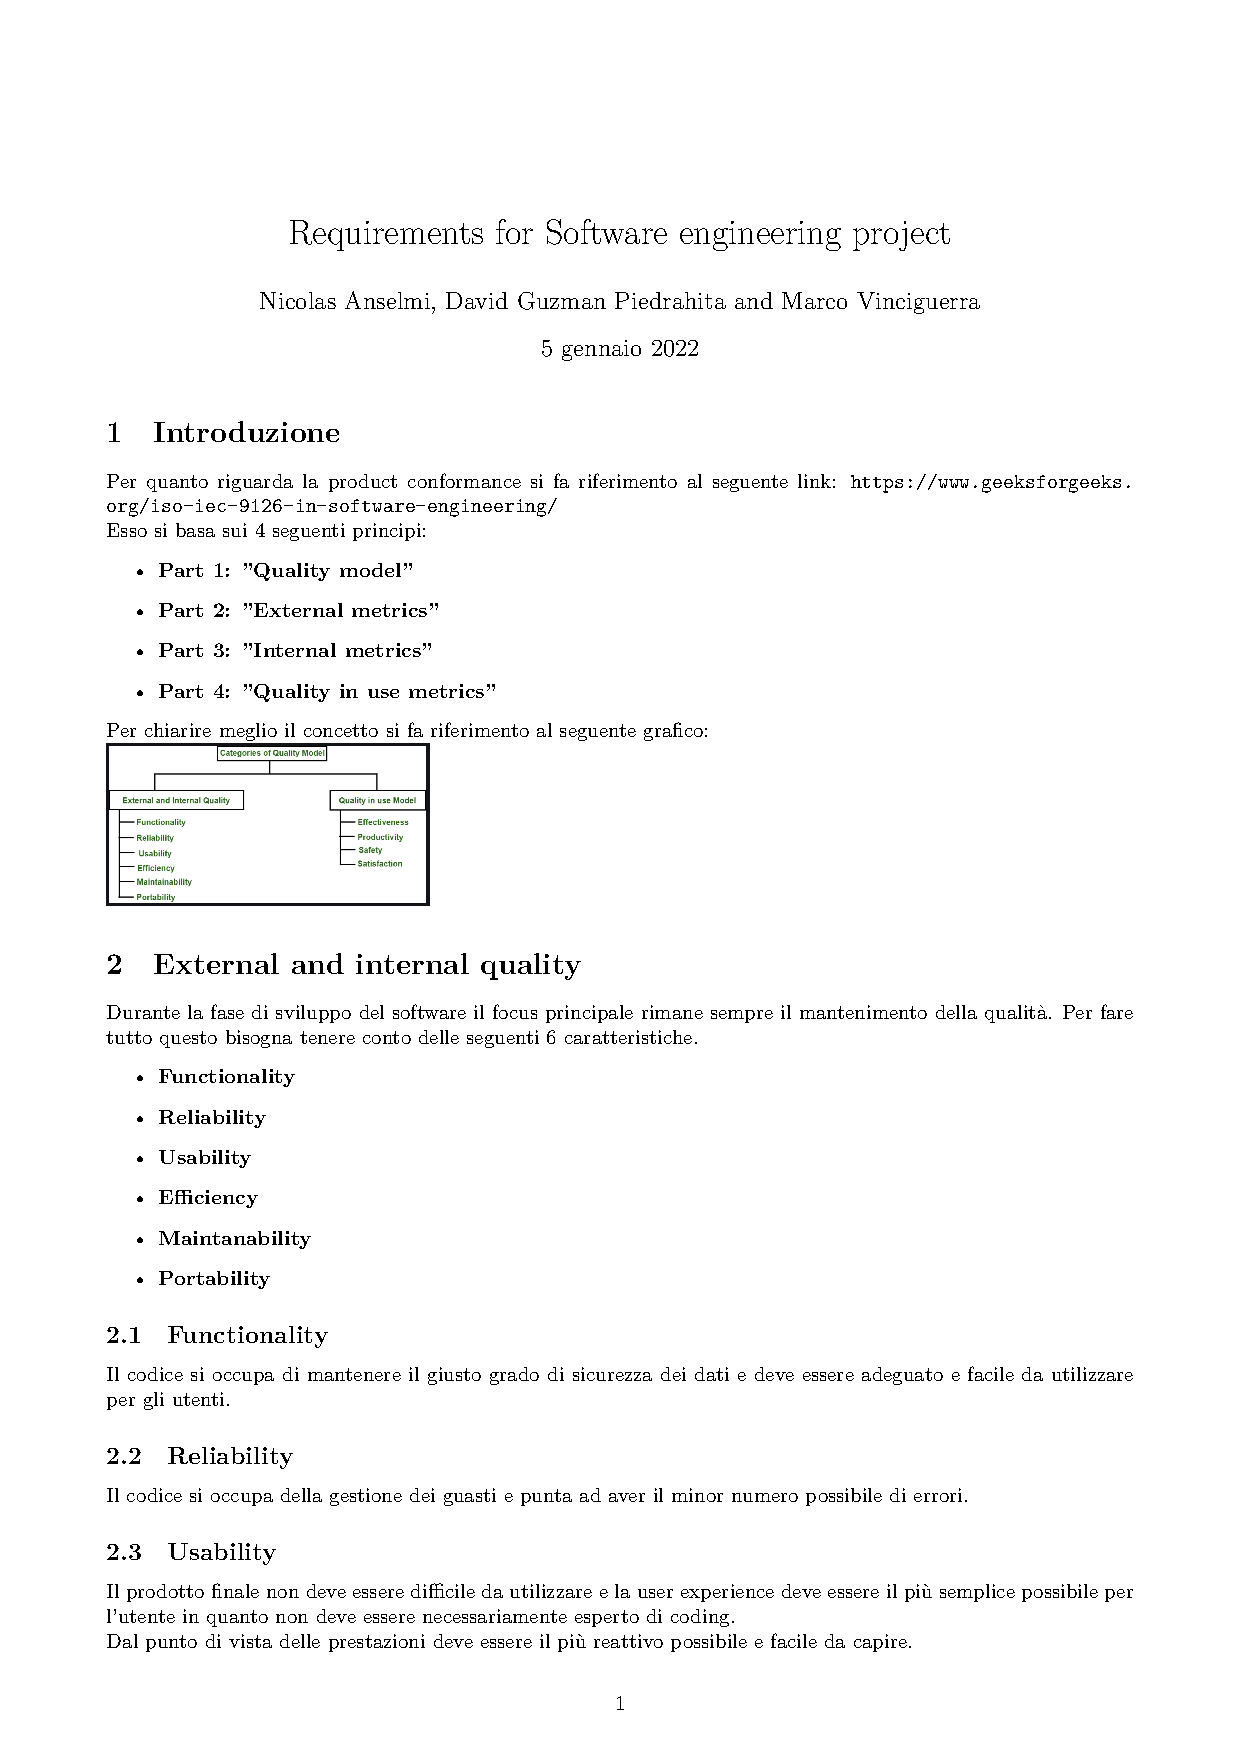
\includegraphics[scale = 0.25]{"Immagini/ISO9126.PNG"}
\section{External and internal quality}
Durante la fase di sviluppo del software il focus principale rimane sempre il mantenimento della qualità.
Per fare tutto questo bisogna tenere conto delle seguenti 6 caratteristiche.
\begin{itemize}
    \item \textbf{Functionality} 
    \item \textbf{Reliability} 
    \item \textbf{Usability} 
    \item \textbf{Efficiency} 
    \item \textbf{Maintanability} 
    \item \textbf{Portability} 
\end{itemize}

\subsection{Functionality}
Il codice si occupa di mantenere il giusto grado di sicurezza dei dati e deve essere adeguato e facile
da utilizzare per gli utenti.

\subsection{Reliability}
Il codice si occupa della gestione dei guasti e punta ad aver il minor numero possibile di errori.

\subsection{Usability}
Il prodotto finale non deve essere difficile da utilizzare e la user experience deve essere il più
semplice possibile per l'utente in quanto non deve essere necessariamente esperto di coding.
\\Dal punto di vista delle prestazioni deve essere il più reattivo possibile e facile da capire.

\subsection{Efficiency}
Si vuole creare il programma più efficiente possibile che utilizzi il minimo delle risorse del dispositivo
da cui si utilizza l'applicazione.

\subsection{Maintanability}
Il codice deve essere scritto nel modo più conforme alle regole di standard di programmazione per favorire
la leggibilità e la successiva manutenzione.

\subsection{Portability}
Il programma deve funziona su più piattaforme possibilil.

\section{Quality in use Model}
Si basa sulle seguenti 4 caratteristiche:
\begin{itemize}
    \item Effectiveness
    \item Productivity
    \item Safety
    \item Satisfaction
\end{itemize}

\end{document}
